\chapter{Mathematical foundations}

Now that we have introduced some preliminary concepts in quantum mechanics and quantum computation, we can turn to the \tbf{mathematical foundations} that will allow us to develop a deeper understanding of the tools ahead. By the end of this chapter, we will be ready to state the postulates of quantum mechanics in a precise form. To prepare for that, we must first lay out several essential definitions and structures.

We will start our mathematical discussion with the definition of \tbf{scalar product} --- we will assume the definitions of vector space, basis and linear independence are already known by the reader.

\begin{frameddefn}{Scalar product}
	Given a scalar product vector space $V$, a \tbf{scalar product} $$\funcmap{\braket{\cdot , \cdot }}{V \times V}{\C}{(v, w)}{\braket{v,w}}$$ is a linear function that satisfies the following properties:

	\begin{itemize}
		\item $\forall u, v, w \in V, \alpha, \beta \in \C \quad \braket{u,\alpha v + \beta w} = \alpha \abk{u,v} + \beta \abk{u,w}$
		\item $\forall u, v \in V \quad \overline{\braket{u,v}} = \braket{v, u}$ --- where $\overline z$ is the conjugate of $z \in \C$
		\item $\forall u \in V \quad \braket{u, u} \ge 0$ and $\braket{u, u} = 0$ if and only if $u = 0$
	\end{itemize}
\end{frameddefn}

We see that the first property is the \tit{linearity} of the scalar product, while the second property is usually referred to as \tit{conjugate-symmetry}. Scalar products are also called \tit{inner product}, and are used to define many other tools on top of the vector space considered.

\begin{framedprop}{}
	For any scalar product vector space $V$, any scalar product satisfies the following property: $$\forall u, v, w \in V, \alpha, \beta \in \C \quad \braket{\alpha u + \beta v, w} = \overline \alpha \braket{u, w} + \overline \beta \braket{v, w}$$
\end{framedprop}

\begin{proof}
	By the properties of scalar product, the following holds
	\begin{equation*}
		\begin{split}
			\braket{\alpha u + \beta v, w} & = \overline{w, \alpha u + \beta v}                                                     \\
			                               & = \overline{\alpha \braket{w, u} + \beta \braket{w, v}}                                \\
			                               & = \overline \alpha \overline{\braket{w, u}} + \overline \beta \overline{\braket{w, v}} \\
			                               & = \overline \alpha \braket{u, w} + \overline \beta \braket{v, w}
		\end{split}
	\end{equation*}
\end{proof}

In particular, the scalar product that we are going to use for our purposes is defined as shown below.

\begin{frameddefn}{Hermitian product}
	Given a vector space $V$ defined over $\C$, the \tbf{Hermitian product} is defined as follows: $$\forall u, v \in \C^n \quad \braket{u, v} = \sum_{i = 1}^n{\overline{u_i} v_i}$$
\end{frameddefn}

\begin{framedprop}{}
	The Hermitian product is a scalar product.
\end{framedprop}

\begin{proof}
	It suffices to prove all the properties of scalar products provided in the definition. Then, we see that

	\begin{itemize}
		\item linearity can be proved as follows $$\braket{u, \alpha v + \beta w} = \sum_{i = 1}^n{\overline{u_i} (\alpha v_i + \beta w_i)} = \alpha\sum_{i = 1}^n{\overline{u_i} v_i} + \beta \sum_{i = 1}^n{\overline{u_i} v_i} = \alpha \braket{u, v} + \beta \braket{u, w}$$
		\item conjugate-symmetry can be shown as follows $$\overline{\braket{v, u}} = \overline{\sum_{i = 1}^n{\overline{v_i} u_i}} = \sum_{i = 1}^n{\overline{\overline{v_i} u_i}}= \sum_{i = 1}^n{v_i \overline{u_i}} = \braket{u, v}$$
		\item lastly, we have that $$\braket{u, u} = \sum_{ i= 1}^n{\overline{u_i}u_i} = \sum_{i = 1}^n{\abs{u_i}^2} \ge 0$$ and clearly it is equal to 0 if and only if $u = 0$
	\end{itemize}
\end{proof}

From now on, when we refer to a \curlyquotes{scalar product} we will refer to the Hermitian product.

We are finally ready to explain the \curlyquotes{braket} that we used from the beginning of the previous chapter. This notation was invented by the Nobel Prize in Physics \href{https://it.wikipedia.org/wiki/Paul_Dirac}{Paul Dirac}, and it works as follows: first, observe that our scalar product can be rewritten as follows $$\braket{u, v} = \rmat{\overline{u_1} \cdots \overline{u_n}} \rmat{v_1 \\ \vdots \\ v_n}$$ To be precise, this product would yield a $1 \times 1$ matrix, which can be interpreted as a scalar. Through Dirac notation, we will write $$\braket{u, v} = \braket{u | v}$$ where $\bra u$ is called \tbf{bra}, and $\ket v$ is called \tbf{ket} (as in \curlyquotes{bra-ket}). In other words, we have that $\ket v$ is just a regular column vector $v \in V$ $$\ket v = \rmat{v_1 \\ \vdots \\ v_n}$$ defined over some scalar product vector space $V$, while $\bra u$ is a \tit{linear map} that acts as follows: $$\funcmap{\bra \cdot}{V}{\overline V}{\rmat{u_1 \cdots u_n}}{\rmat{\overline{u_1} \cdots \overline{u_n}}}$$ We observe that from this very definition we can already see the power of the Dirac notation: by writing $$\bra u \cdot \ket v$$ we are writing the product between a row conjugated vector $u$ and a column vector $v$, which will ultimately yield $1 \times 1$ vector containing exatcly $\braket{u, v}$! Therefore, this allows us to write that $$\bra u \cdot \ket v = \braket{u|v}$$

\begin{framedthm}[label={cs ineq}]{Cauchy-Schwarz inequality}
	Given a scalar product vector space $V$, it holds that $$\forall u, v \in V \quad \abs{\braket{u|v}} \le \sqrt{\braket{u|u} \braket{v|v}}$$ where the equality holds if and only if $u$ and $v$ are linearly independent.
\end{framedthm}

Moreover, our scalar product induces a \tbf{norm}, which is defined as follows.

\begin{frameddefn}{Norm}
	Given a scalar product vector space $V$, the \tbf{norm} of a vector $v \in V$ is defined as follows $$\norm v = \sqrt{\braket{v|v}}$$
\end{frameddefn}

As usual, two vectors $u, v \in V$ are said to be \tbf{orthogonal} if $\braket{u|v} = 0$. This allows us to define orthonormal bases.

\begin{frameddefn}{Orthonormal basis}
	Given a scalar product vector space $V$, a basis $\{e_1, \ldots, e_n\}$ is said to be \tbf{orthonormal} if $$\forall i, j \in [n] \quad \braket{e_i | e_j} = \delta_{ij}$$ where $\delta_{ij} = \soe{ll}{1 & i = j \\ 0 & i \neq j}$ is called \tbf{Kronecker delta}.
\end{frameddefn}


Let's see the Dirac notation in action. Consider an orthonormal basis $\{e_1, \ldots, e_n\}$ for some scalar product vector space $V$; by definition, we know that we can write any vector $u \in V$ as follows $$u = \sum_{i = 1}^n{\alpha_i e_i}$$ for some coefficients $\alpha_1, \ldots, \alpha_n \in \C$. Now, we observe that for all $i \in [n]$
\begin{equation*}
	\begin{alignedat}{2}
		\braket{e_i|u} & = \abk{e_i\middle|\sum_{j = 1}^n{\alpha_j e_j}}                      & \\
		               & = \abk{e_i \middle|\alpha_1e_1 + \ldots + \alpha_n e_n}          & \\
		               & = \alpha_1 \braket{e_i|e_1} + \ldots + \alpha_n \braket{e_i|e_n} & \\
		               & = \sum_{j = 1}^n{\alpha_j\braket{e_i | e_j}}                     & \\
		               & = \sum_{j = 1}^n{\alpha_j \delta_{ij}}                           & \\
		               & = \alpha_i                                                       & \\
	\end{alignedat}
\end{equation*}
Indeed, with the scalar product we can compute the projection of $u$ onto the $i$-th vector of the basis. Hence, we can rewrite the first equation as follows: $$\ket u = \sum_{i = 1}^n{\alpha_i \ket{e_i}} = \sum_{i = 1}^n{\braket{e_i|u} \ket{e_i}}$$ In particular, we observe that $$\ket u = \sum_{i = 1}^n{\ket{e_i} \braket{e_i|u}} \implies I = \sum_{i = 1}^n{\ket{e_i} \bra{e_i}}$$ which is a famous identity in quantum mechanics called \tbf{resolution of the identity}. In particular, this identity directly implies the following useful property. As a final note, by the properties of scalar products we also have that $$\braket{v|u} = \bra{v} \sum_{i = 1}^n{\ket{e_i} \braket{e_i|u}} = \sum_{i= 1}^n{\braket{v|e_i} \braket{e_i|u}}$$

\begin{framedprop}{}
	Given a scalar product vector space $V$, it holds that $$\forall u, v, w \in V \quad \braket{u|v} \ket w = (\ket w \bra u) \ket v$$
\end{framedprop}

\section{Hilbert spaces}

Now that we covered Dirac notation, we can describe what are \tbf{Hilbert spaces} --- we will see why we care about this particular type of vector spaces later in the chapter. First, consider the following definitions.

\begin{frameddefn}{Weak convergence}
	Given a scalar product vector space $V$, and a vector sequence $\{v_m\}_{m \in \N}$ defined over $V$, we say that the sequence \tbf{converges weakly} to a vector $v \in V$ if $$\forall w \in V \quad \lim_{m \to + \infty}{\braket{v_m|w}} = \braket{v|w}$$
\end{frameddefn}

In other words, this type ocf convergence requires all projections of $v_m$ along any fixed direction $w$ to approach the projection of $v$. Differently, the next type of convergence is more strict.

\begin{frameddefn}{Strong convergence}
	Given a scalar product vector space $V$, and a vector sequence $\{v_m\}_{m \in \N}$ defined over $V$, we say that the sequence \tbf{converges strongly} to a vector $v \in V$ if $$\lim_{m \to + \infty}{\norm{v - v_m}} = 0$$
\end{frameddefn}

In fact, this type of convergence requires the actual vectors of the sequence to get close \tit{in norm} to $v$. We observe the following proposition.

\begin{framedprop}{}
	Given a scalar product vector space $V$, and a vector sequence $\{v_m\}_{m \in \N}$ defined over $V$, if the sequence converges strongly to some vector $v \in V$, it holds that

	\begin{itemize}
		\item the sequence also converges weakly
		\item the scalar products defined over $V$ are continuous, i.e. $$\forall u, v \in V \quad \braket{u|v} = \lim_{m \to + \infty}{\braket{u|v_m}}$$
	\end{itemize}
\end{framedprop}

\begin{frameddefn}{Cauchy sequence}
	Given a scalar product vector space $V$, and a vector sequence $\{v_m\}_{m \in \N}$ defined over $V$, we say that the sequence is a \tbf{Cauchy sequence} if it holds that $$\forall \varepsilon > 0 \quad \exists n_\varepsilon \in \N \quad \forall n, m > n_\varepsilon \quad \norm{v_n - v_m} < \varepsilon$$
\end{frameddefn}

For example, let's consider the space $\R^2$ equipped with the Euclidean norm $$\norm v =  \sqrt{x^2 + y^2}$$ Then, if we consider the following vector sequence $$\cbk{\rmat{\tfrac{1}{m} \\ \vdots \\ \tfrac{1}{m}}}_{m \in \N}$$ we see that for any distinct $m, n$ it holds that $$\norm{v_m - v_n} = \sqrt{\rbk{\dfrac{1}{m} -\dfrac{1}{n}}^2 + \rbk{\dfrac{1}{m} -\dfrac{1}{n}}^2} = \sqrt 2 \abs{\dfrac{1}{m} -\dfrac{1}{n}}$$ Therefore, for any $\varepsilon > 0$ it suffices to take any $N > \dfrac{2 \sqrt 2}{\varepsilon}$ such that $$\forall m, n > N \quad \norm{v_m - v_n} < \varepsilon$$

We are finally ready to define Hilbert spaces.

\begin{frameddefn}{Hilbert space}
	A \tbf{Hilbert space} is a \tit{complete} scalar product vector space, i.e. it is a vector space

	\begin{itemize}
		\item equipped with a scalar product
		\item such that every Cauchy sequence converges strongly to an element in the space.
	\end{itemize}
\end{frameddefn}

For example, the space $\R^n$ is a Hilbert space. Indeed, since every finite vector space of size $n$ is isomporphic to $\R^n$, we can immediately derive the following proposition.

\begin{framedprop}{}
	Finite-dimensional vector spaces are always complete.
\end{framedprop}

\subsection{Linear operators}

Given a Hilbert space $\mathcal H$, we can define \tbf{operators} --- which are nothing but linear maps.

\begin{frameddefn}{Adjoint operator}
	Given a Hilbert space $\mathcal H$, and an operator $A$, the \tbf{adjoint} operator of $A$, denoted with $A^\dag$, is a linear map that satisfies the following property $$\forall u, v \in \mathcal H \quad \braket{u|A^\dag v} = \braket{Au|v}$$ We say that an operator $A$ is \tbf{self-adjoint}, or \tit{Hermitian}, if and only if $A = A^\dag$.
\end{frameddefn}

For instance, the following matrix $S = \rmat{1 & 0 \\ 0 & i}$ is a linear operator whose adjoint is $S^\dag = \rmat{1 & 0 \\ 0 & -i}$. In fact, we have that $$\braket{u|S^\dag v} = \rmat{\overline{u_1} & \overline{u_2}} \rmat{1 & 0 \\ 0 & -i} \rmat{v_1 \\ v_2} = \rmat{\overline{u_1} & \overline{u_2}} \rmat{v_1 \\ -iv_2} = \overline{u_1}v_1 - i\overline{u_2}v_2$$ and since $$Su = \rmat{1 & 0 \\ 0 & i}\rmat{u_1 \\ u_2} = \rmat{u_1 \\ iu_2} \implies \bra{Su} = \rmat{\overline{u_1} & \overline{i u_2}}$$ but because $\overline{iu_2} = \overline i \cdot \overline{u_2} = -i \overline{u_2}$ this implies that $$\braket{Su |v} = \rmat{\overline{u_1} & -i\overline{u_2}} \rmat{v_1 \\ v_2} = \overline{u_1}v_2 - i\overline{u_2}v_2$$

\begin{framedprop}[label={adj prop}]{}
	For any adjoint operators $A, B$ defined over some Hilbert space $\mathcal H$, it holds that

	\begin{enumerate}
		\item $(AB)^\dag = B^\dag A^\dag$
		\item for any scalar $z$ it holds that $(zA)^\dag = \overline z A^\dag$
		\item $(A^\dag)^\dag = A$
		\item $(A + B)^\dag = A^\dag + B^\dag$
	\end{enumerate}
\end{framedprop}

How do we evaluate the adjoint of a given operator?

\begin{framedprop}[label={conj transp}]{}
	Given an operator $A$ defined over a scalar product vector space, it holds that $$a_{ij}^\dag = \overline{a_{ji}}$$
\end{framedprop}

This property is incredibly useful, because it implies that the adjoint operator of $A$ is its transposed conjugate matrix. Most notably, due to the way we defined our scalar product, it holds that for any column vector $\ket x$ we have that $$\bra x = \ket x^\dag$$ which gives an intuition of the reason why we defined our scalar product as such.

\begin{frameddefn}{Positive operator}
	An operator $A$ defined over a scalar product vector space $\mathcal H$ is said to be \tbf{positive} if it holds that $$\forall v \in \mathcal H \quad \braket{v|Av} \ge 0$$
\end{frameddefn}

\begin{framedprop}[label={positive prop}]{}
	If an operator $A$ is positive, then it is Hermitian.
\end{framedprop}

\begin{proof}
	TODO \todo{la dimostrazione che ha scritto lui è sbagliata}
\end{proof}

% \begin{proof}
% 	Let $A$ be a positive operator, therefore $$\forall v \in \mathcal H \quad \braket{v|Av} \ge 0$$ We observe that if $\braket{v|Av} \ge 0$, this implicitly means that $\braket{v|Av}$ is a real value. This is important because then $$\forall v \in \mathcal H \quad \braket{v|Av} = \overline{\braket{v|Av}}$$ From this, we derive the following
% 	\begin{equation*}
% 		\begin{split}
% 			\forall v \in \mathcal H \quad \overline{\braket{v|Av}} & = \braket{v|Av}                  \\
% 			                                                        & = \braket{A^\dag v|v}            \\
% 			                                                        & = \overline{\braket{v|A^\dag v}}
% 		\end{split}
% 	\end{equation*}
% 	which implies that $$\forall v \in \mathcal H \quad \braket{v|Av} = \braket{v|A^\dag v}$$ Now, consider the following claim.
%
% 	\claim{
% 		If $\braket{x|z} = \braket{y|z}$ for all $z \in \mathcal H$, then $x = y$.
% 	}{
% 		Fix a vector $z \in \mathcal H$; we observe that
% 		\begin{equation*}
% 			\begin{split}
% 				     & \braket{x|z} = \braket{y|z}     \\
% 				\iff & \braket{x|z} - \braket{y|z} = 0 \\
% 				\iff & (\bra x - \bra y) \ket z = 0    \\
% 				\iff & \braket{x - y|z} = 0
% 			\end{split}
% 		\end{equation*}
% 		However, if this is true for every vector $z \in \mathcal H$ it means that the vector $x - y$ is orthogonal to every vector in $\mathcal H$, which must imply that $x - y$ is the 0 vector, thus $$x - y = 0 \iff x = y$$
% 	}
%
% 	From this claim, we have that $$\forall v \in \mathcal H \quad \braket{v|Av} = \braket{v|A^\dag v} \iff \braket{A^\dag v|v} = \braket{Av|v} \implies A^\dag v = Av$$ which implies that $A$ must be Hermitian.
% \end{proof}

At the beginning of the previous chapter we said that all quantum gates are \tit{unitary transformations}, but we did now provide a definition of unitary. Now we are ready to introduce it, and start to grasp why we are discussing Hilbert spaces.

\begin{frameddefn}{Unitary operators}
	Given a Hilbert space $\mathcal H$, and an operator $U$, we say that $U$ is \tbf{unitary} if it holds that $$UU^\dag = U^\dag U = I$$
\end{frameddefn}

In other words, $U$ is unitary if and only if its adjoint operator is also its inverse. An interesting characterization of unitary transformations is the following property.

\begin{framedprop}[label={unitary alt def}]{Unitary operators (alt. def.)}
	An operator $U$ defined over a Hilbert space $\mathcal H$ is unitary if and only if

	\begin{itemize}
		\item $U$ is surjective
		\item $\forall x, y \in \mathcal H \quad \braket{Ux|Uy} = \braket{x|y}$ or equivalently, if it holds that $$\forall x \in \mathcal H \quad \norm{Ux} = \norm x$$
	\end{itemize}
\end{framedprop}

\begin{proof}
	TODO \todo{TODO}
\end{proof}

In particular, we observe that the second property of this proposition is very interesting: the \tit{preservation of the scalar product}, i.e. the property for which $$\forall x, y \in \mathcal H \quad \braket{Ux|Uy} = \braket{x|y}$$ means that the operator $U$ does not change the geometric relationships between vectors --- i.e. their lengths and angles remain the same.

\begin{framedprop}[label={rows cols unit}]{}
	If $U$ is a unitary operator, then the rows and the columns of $U$ are orthonormal.
\end{framedprop}

\begin{proof}
	First, we prove that the rows and columns of $U$ are normalized.

	\claim[Claim 1]{
		The norm of the rows and the columns of $U$ is 1.
	}{
		By the previous proposition, we know that $$\forall x \in \mathcal H \quad \norm{Ux} = \norm x$$ and in particular, this must hold for the canonical basis as well. This means that $$\norm{Ue_i} = \norm{e_i} = 1$$ for any vector of the canonical basis $e_i$. Then, since $Ue_i$ is just the $i$-th column of $U$, this proves that each column of $U$ has norm1.

		To prove the same result for the rows, observe that by \cref{conj transp} it holds that $$U^\dag = \overline U ^T$$ and \todo{da finire boh come??}
	}

	Next, we show orthogonality of rows and columns.

	\claim[Claim 2]{
		The rows and columns of $U$ are orthogonal.
	}{
		By the preservation of the scalar product, we know that $$\forall x, y \in \mathcal H \quad \braket{Ux|Uy} = \braket{x|y}$$ and in particular, this must also hold for the canonical basis. This means that for any pair of vectors of the canonical basis we have that $$\forall i, j \quad \braket{Ue_i|Ue_j} = \braket{e_i|e_j} = \delta{ij}$$ which means that the rows and columnds of $U$ must be orthogonal. \todo{does it?}
	}

	The two claims together conclude the proof.
\end{proof}

\begin{framedprop}[label={unitary prod}]{}
	If $A$ and $B$ are two unitary operators, then $AB$ is a unitary operator.
\end{framedprop}

\begin{proof}
	Since $A$ and $B$ are unitary it holds that $$A ^\dag A = A A^ \dag = B ^ \dag B = B B^ \dag = I$$ Now, by \cref{adj prop} we have that $$(AB)^ \dag = B^\dag A^\dag$$ from which we conclude that $$(AB)^\dag(AB) = B^\dag A^\dag AB = B^\dag I B = B^\dag B = I$$
\end{proof}

\begin{frameddefn}{Normal operators}
	Given a Hilbert space $\mathcal H$, and an operator $A$, we say that $A$ is \tbf{normal} if it satisfies the following property $$A^\dag A = AA^\dag$$
\end{frameddefn}

Clearly, from their definition we immediately see that both self-adjoint and unitary operators are both normal.

Lastly, say that we know that how an operator $U$ acts on some input $\ket x$, and we want to derive $U$. How can we do this?

\begin{framedprop}[label={U constr}]{}
	For any operator $U$ in a Hilbert space $\mathcal H$, if $\mathcal B$ is a base of $\mathcal H$ it holds that $$U = \sum_{b \in \mathcal B}{U \ket b \bra b}$$
\end{framedprop}

\begin{proof}
	The formula derives directly from the resolution of the identity, and the linearity of operators of Hilbert spaces
	\begin{equation*}
		\begin{split}
			U & = U \cdot I                                      \\
			  & = U \cdot \sum_{b \in \mathcal B}{\ket b \bra b} \\
			  & = \sum_{b \in \mathcal B}{U \ket b \bra b}
		\end{split}
	\end{equation*}
\end{proof}

Therefore, if we know how $U$ acts component-wise, we can reconstruct the operator acting on the whole space as such.

To conclude this section, we introduce a definition that will be very useful in the next chapter.

\begin{frameddefn}{Trace}
	Given a matrix $A \in \C^{n \times n}$, its \tbf{trace} is defined as follows: $$\tr(A) := \sum_{i = 1}^n{a_{ii}}$$
\end{frameddefn}

In other words, the trace of a matrix is the sum of the elements on its diagonal.

\begin{framedprop}[label={trace tricks}]{}
	Given two matrices $A, B \in \C^{n \times n}$, it holds that

	\begin{enumerate}
		\item $\tr(AB) = \tr(BA)$, meaning that the trace is \tit{cyclic}
		\item $\tr(A + B) = \tr(A) + \tr(B)$, meaning that the trace is \tit{linear}
		\item $\forall z \in \C \quad \tr(zA) = z \tr(A)$
		\item $\tr(A) = \tr(UAU^\dag)$ if $U$ is unitary, meaning that the trace is \tit{invariant under unitary similarity transformation}
	\end{enumerate}
\end{framedprop}

In particular, we observe that the last property follow trivially from the cyclic property: $$\tr(UAU^\dag) = \tr(UU^\dag A) = \tr(I A) = \tr(A)$$ But perhaps most importantly, the following property holds.

\begin{framedprop}[label={trace prop}]{}
	Given a matrix $A \in \C^{n \times n}$, and a vector $\ket v$, it holds that $$\tr(A \ket v \bra v) = \braket{v|Av}$$
\end{framedprop}

\begin{proof}
	First, we observe that the definition of the trace can be rewritten in terms of the Dirac notation $$\tr(X) = \sum_{i = 1}^n{x_{ii}} = \sum_{i = 1}^n{\braket{e_i|X|e_i}}$$ From this equality, we conclude that
	\begin{equation*}
		\begin{split}
			\tr(A \ket v \bra v) & = \sum_{i = 1}^n{\braket{e_i|A|v} \braket{v|e_i}}             \\
			                     & = \sum_{i = 1}^n{\braket{\psi|e_i} \braket{e_i|A|v}}          \\
			                     & = \bra{v} \rbk{\sum_{i = 1}^n{\ket {e_i} \bra{e_i}}} A \ket v \\
			                     & = \braket{v|A|v}                                              \\
			                     & = \braket{v|Av}
		\end{split}
	\end{equation*}
\end{proof}

Most importantly, if we set $A$ to be the identity matrix, we obtain an interesting identity: $$\tr( \ket v \bra v) = \braket{v|v}$$ which should not come as a surprise anyway, since the elements on the diagonal of $\ket v \bra v$ as exactly the elements of the sum in the scalar product of $\braket{v|v}$. We will discuss the importance of this equality in later sections.

TODO \todo{show that the trace is indep of the chosen basis}

\section{Spectral theory}

Since unitary operators are linear maps, we are interested in their eigenvectors and eigenvalues --- which are defined as usual. First, let us recall some preliminary definitions.

\begin{frameddefn}{Non-degenerate eigenvalue}
	Given a matrix $A$, and an eigenvalue $\lambda$ of $A$, we say that $\lambda$ is \tbf{non-degenerate} if the associated eigenspace has dimension 1 (or equivalently, if it has only 1 associated eigenvector).
\end{frameddefn}

\begin{frameddefn}{$d$-fold degenerate eigenvalue}
	Given a matrix $A$, and an eigenvalue $\lambda$ of $A$, we say that $\lambda$ is $d$-fold degenerate if there are $d$ linearly independent eigenvectors $u_1, \ldots, u_d$ associated to $\lambda$.
\end{frameddefn}

In Dirac notation, if $\lambda$ is non-degenerate, we refer to the only eigenvector associated to $\lambda$ as $\ket \lambda$, indeed it holds that $$A \ket \lambda = \lambda \ket \lambda$$ Interestingly enough from this equation we can immediately derive the following equality as well $$\bra \lambda A^\dag = \overline \lambda \bra \lambda$$

The following theorem provides a characterization of the eigenvalues and eigenvectors of self-adjoint and unitary operators, which have surprisingly nice properties.

\begin{framedthm}[label={spectral thm}]{Spectral theorem}
	The following propositions hold:

	\begin{itemize}
		\item The eigenvalues of a self-adjoint operator are real values.
		\item The eigenvalues of a unitary operator are complex values of modulus 1.
		\item Eigenvectors of self-adjoint and unitary operators associated to different eigenvalues are orthogonal to each other.
	\end{itemize}
\end{framedthm}

Moreover, for finite-dimensional Hilbert spaces the following holds.

\begin{framedthm}[label={spectral thm 2}]{Spectral theorem for fin. Hilbert spaces}
	Given a finite-dimensional Hilbert space $\mathcal H$, and a normal operator $A$ defined over $\mathcal H$, the set of all eigenvectors of $A$ can be expanded to form an orthonormal basis for $\mathcal H$.
\end{framedthm}

In particular, to basis expansion can be achieve through the \tbf{Gram-Shmidt} in the each degenerate eigenspace of $A$ in order to produce an orthonormal set.

% We can rewrite this thorem as follows: if we denote with $u_{ij}$ the $j$-th eigenvector associated to the $i$-th eigenvalue of $A$, it holds that $$\forall v \in \mathcal H \quad v = \sum_{i = 1}^m{\sum_{j = 1}^{d_i}{\alpha_{ij} u_{ij}}}$$ where $d_i$ is the geometric multiplicity of the $i$-th eigenvalue of $A$. Indeed, we observe that $\dim \mathcal H = \sum_{i = 1}^m{d_i}$. Lastly, through the Dirac notation we can rewrite the formula as follows $$\forall v \in \mathcal H \quad \ket v = \sum_{i = 1}^m{\sum_{j = 1}^{d_i}{\braket{\lambda_{ij}|v} \ket{\lambda_{ij}}}}$$

\section{Projectors}

Next, we are going to discuss \tbf{projectors}, which are another very crucial pieces of quantum computation. We saw how scalar products are able to perform projection over desired direction, in fact we will use the Dirac notation to define precise operators for our purposes. But as always, first some preliminary definitions.

\begin{frameddefn}{Orthogonal space}
	Given a scalar product vector space $U$, and two linear subspaces $V, W \subset U$, we say that $V$ is orthogonal to $W$ if $$\forall v \in V, w \in W \quad \braket{v|w} = 0$$
\end{frameddefn}

Given a scalar product vector space $U$, and a linear subspace $V \subset U$, the \tbf{orthogonal complement} of $V$ is defined as follows: $$V^\bot := \{u \in U \mid \forall v \in v \quad \braket{u|v} = 0\}$$ In particular, we observe that if $U$ is finite-dimentional it holds that $V = U - V^\bot$ and that $(V^\bot)^\bot = V$.

\begin{frameddefn}{Topologically closed subspace}
	Given a Hilbert space $\mathcal H$, and a linear subspace $V \subset \mathcal H$, we say that $V$ is \tbf{topologically closed} if any sequence of vectors defined over $V$ converges in $V$.
\end{frameddefn}

Interestingly enough, given a topologically closed subspace $V \subset \mathcal H$ of some Hilbert space, we can write any vector $u \in V$ as the sum of two orthogonal vectors of $V$ and $V^\bot$, as follows. Let $\{f_1, \ldots, f_n\}$ be an orthonormal basis of $V$, and define the following vectors $$\forall u \in U \quad u_V := \sum_{i = 1}^n{\braket{f_i|v} f_i}$$ Then, if we call $$u_{V^\bot} := u - u_V$$, we see that
% \begin{equation*}
%     \begin{alignedat}{2}
%         \braket{u_V|u_{V^\bot}} &= \braket{u_V|u - u_V} & \\ 
%                                 &= \braket{u_V|u} - \braket{u_V|u_V} & \\ 
%                                 &= \braket{\sum_{i = 1}^n{\braket{f_i|u} f_i}|u} - \braket{u_V|u_V} & \\ 
%                                 &= \sum_{i = 1}^n{\braket{f_i|u} \braket{f_i|u}} - \braket{u_V|u_V} & \\ 
%                                 &= \sum_{i = 1}^n{\abs{\braket{f_i|u}}^2} - \braket{u_V|u_V} & \\ 
%                                 &= \sum_{i = 1}^n{\overline{\braket{f_i|u}} \braket{f_i|u}} & \quad (\mbox{since $\abs{z}^2 = z \cdot \overline z$}) \\ 
%                                 & = \sum_{i = 1}^n{\sum_{j = 1}^n{\overline{\braket{f_i|u}} \braket{f_j|u} \delta_{i j}}} & \quad (\mbox{since $\delta_{ij} = \braket{f_i|f_j}$})
%     \end{alignedat}
% \end{equation*}
TODO \todo{decommenta e finisci la formula} which indeed proves that $u_V$ and $u_{V^\bot}$ are orthogonal to each other.

With this observation, we can finally define the projector operators.

\begin{frameddefn}{Projector}
	Given a Hilbert space $\mathcal H$, and a closed subspace $V \subset \mathcal H$, the \tbf{projector} operator that projects any given vector $v \in \mathcal H$ onto $V$ is defined as follows: $$\funcmap{P_V}{\mathcal H}{V}{u}{u_V = \sum_{i = 1}^n{\braket{f_i|u} f_i}}$$ where $\{f_1, \ldots, f_n\}$ is an orthonormal basis of $V$.
\end{frameddefn}

Most importantly, given the map in the definition we have that the projector operator $P_V$ is defined as follows $$P_V := \sum_{i = 1}^n{\ket{f_i} \bra{f_i}}$$ Clearly, by definition of $u_{V^\bot}$ it holds that $$\funcmap{P_{V^\bot}}{\mathcal H}{V^\bot}{u}{u_{V^\bot} := u - u_V}$$ Moreover, since $P_V$ performs a projection, we have that $$\forall u \in \mathcal H \quad u \in V \iff P_Vu = u$$ and that $$\forall u \in \mathcal H \quad u \in V^\bot \iff P_V u = 0$$

\begin{framedthm}{characterization of projectors}
	Given a Hilbert space $\mathcal H$, an operator $P_V$ is the projector on some closed subspace $V \subset \mathcal H$ if and only if
	\begin{enumerate}
		\item $P_V^2 = P_V$, i.e. it is \tit{idempotent}
		\item $P_V^\dag = P_V$, i.e it is Hermitian
	\end{enumerate}
\end{framedthm}

\begin{proof}
	We first prove the direct implication. Suppose that $P_V$ is the projector of a vector space $V \subset \mathcal H$, meaning that $P_V$ can be written as $$P_V = \sum_{i = 1}^n \ket {f_i} \bra{f_i}$$ for some orthonormal basis $\{f_i\}_{i = 1}^n$ of $V$. Then, we observe that
	\begin{equation*}
		\begin{split}
			P_V^2 & = \rbk{\sum_{i = 1}^n \ket{f_i} \bra{f_i}} \rbk{\sum_{j = 1}^n \ket{f_j} \bra{f_j}} \\
			      & = \sum_{i = 1} ^n \sum_{j = n} \ket{f_i} \braket{f_i|f_j} \bra{f_j}                 \\
			      & = \sum_{i = 1}^n \sum_{j = n} \ket{f_i} \delta_{i, j} \bra{f_j}                     \\
			      & = \sum_{i = 1}^n \ket{f_i} \bra{f_i} \\ 
			      & = P_V
		\end{split}
	\end{equation*}
	which immediately proves the idempotency of $P_V$. To prove Hermiticity, we observe that for any vector $\ket v$ it holds that $$(\ket v \bra v)^\dag = \ket v \bra v$$ that together with \cref{adj prop} it implies that
	\begin{equation*}
		\begin{split}
			P_V^\dag & = \rbk{\sum_{i = 1}^n{\ket{f_i} \bra{f_i}}}^\dag \\
			         & = \sum_{i = 1}^n{(\ket{f_i} \bra{f_i})^\dag}     \\
			         & = \sum_{i = 1}^n{\ket{f_i} \bra{f_i}}            \\
			         & = P_V
		\end{split}
	\end{equation*}
	We prove the converse implication in \cref{converse proj}.
\end{proof}

Given a Hilbert space $\mathcal H$, and two topologically closed subspaces $V, W \subset \mathcal H$, we say that $P_V$ and $P_W$ are \tbf{orthogonal} if it holds that $V \bot W$. Now, fix a vector $u \in \mathcal H$; by definition $P_Vu$ is a vector that lies inside $V$, therefore it holds that $$P_W(P_Vu) = 0$$ since $V \bot W$, and by the same reasoning applied on $W$ first we conclude that $$P_WP_V = P_VP_W = \mathbf 0$$ where $\mathbf 0$ is the \tbf{zero operator} --- indeed, it is a zero matrix.

As a final note, if $A$ is an linear operator, and $\lambda$ is an eigenvalue of $A$, we denote with $P_\lambda$ the projector that projects vectors onto the eigenspace associated to $\lambda$.

\begin{framedprop}[label={projector sum}]{}
	If $P$ and $Q$ are two orthogonal projectors, then $P + Q$ is a projector.
\end{framedprop}

\begin{proof}
    Let $\{f_i\}_{i = 1}^n$ and $\{g_i\}_{i = 1}^n$ be the bases that define $$P := \sum_{i = 1}^n \ket{f_i}\bra{f_i} \quad \quad Q := \sum_{i = 1}^n \ket{g_i} \bra{g_i}$$ We observe that $P \bot Q$, which means that $$\forall i, j \in [1, n] \quad \braket{f_i|g_j} = 0$$ Then, we have that $$P + Q = \sum_{i = 1} ^n \ket{f_i} \bra{f_i} + \sum_{i = 1}^n \ket{g_i} \bra{g_i}$$ Then, by the previous theorem it suffices to show that $P + Q$ is both idempotent and Hermitian. To prove idempotency we see that
    \begin{equation*}
	\hspace{-0.3cm}
        \begin{alignedat}{2}
            (P + Q)^2 & =  \rbk{\sum_{i = 1}^n \ket{f_i} \bra{f_i} + \sum_{i = 1}^n \ket{g_i} \bra{g_i }} \rbk{ \sum_{j = 1}^n \ket{f_j} \bra{f_j} + \sum_{j = 1}^n \ket{g_j} \bra {g_j}} & \\ 
                      & = \sum_{i, j}\ket{f_i } \braket{f_i|f_j} \bra{f_j} + \sum_{i, j} \braket{f_i} \braket{f_i|g_j} \bra{g_j} + \sum_{i, j} \ket{g_i} \braket{g_i|f_j} \bra{f_j} + \sum_{i, j} \ket{g_i } \braket{g_i|g_j} \bra{g_j} & \\ 
                      & = \sum_{i, j}\ket{f_i } \delta_{i, j} \bra{f_j} + \sum_{i, j} \ket{g_i } \delta_{i, j } \bra{g_j} & \\ 
                      & = \sum_{i = 1}^n \ket{f_i} \bra{f_i} + \sum_{j = 1}^n \ket{g_j} \bra{g_j} & \\ 
                      & = P + Q
        \end{alignedat}
    \end{equation*}
    We observe that we used orthogonality to remove the inner sums in the third step. Moreover, Hermiticity can be easily proven by linearity of the adjoint:
    \begin{equation*}
        \begin{split}
            (P + Q)^\dag & = \rbk{\sum_{i = 1}^n \ket{f_i} \bra{f_i } + \sum_{i = 1}^n \ket{g_i} \bra{g_i } }^\dag\\ 
                         & = \sum_{i = 1}^n (\ket {f_i} \bra{f_i})^\dag + \sum_{i = 1}^n (\ket{g_i} \bra{g_i})^\dag \\
                         & = \sum_{i = 1}^n \ket {f_i} \bra{f_i}+ \sum_{i = 1}^n \ket{g_i} \bra{g_i} \\ 
                          & = P + Q
        \end{split}
    \end{equation*}
\end{proof}

The importance of the next theorem cannot be understated, and it will be used extensively throughout the notes to prove various results.

\begin{framedthm}[label={spectral decomp}]{Spectral decomposition}
	Given a Hilbert space $\mathcal H$, and a normal operator $A$ defined on $\mathcal H$ whose eigenvalues are $\lambda_1, \ldots, \lambda_n$, the matrix $A$ can be rewritten as follows: $$A = \sum_{i = 1}^n{\lambda_i P_{\lambda_i}}$$
\end{framedthm}

The theorem above is sometimes written in the following different form $$A = \sum_{i = 1}^n{\lambda_i \ket{\lambda_i} \bra{\lambda_i}}$$ which \tit{seems} to imply that $P_{\lambda_i} = \ket{\lambda_i} \bra{\lambda_i}$, i.e. the projector onto the $i$-th eigenspace of $M$ is $\ket{\lambda_i} \bra{\lambda_i}$. This is a \tit{slight} notation abuse, and an example will make it clear. Consider the following matrix: $$A = \rmat{2 & 0 & 0 \\ 0 & 2 & 0 \\ 0 & 0 & 5}$$ It is easy to see that the eigenvalues of $A$ are only 2 and 5, however 2 is $2$-fold degenerate! Indeed, by solving $$M \ket v = 2 \ket v$$ we get an eigenspace of dimension 2, and we can choose $\{\ket {e_1}, \ket {e_2}\}$ as orthonormal eigenbasis; similarly, we find that $\{\ket {e_3}\}$ is an eigenbasis of the second eigenspace of dimension 1. In the end, this means that
\begin{equation*}
	\begin{split}
		M & = 2 \ket 1 \bra 1 + 2 \ket 2 \bra 2 + 5 \ket 3 \bra 3 \\
		  & = 2 (\ket 1 \bra 1 + \ket 2 \bra 2) + 5 \ket 3 \bra 3 \\
		  & = 2 P_2 + 5 P_5                                       \\
	\end{split}
\end{equation*}
which clearly shows that, in general, $P_{\lambda_i} \neq \ket{\lambda_i} \bra{\lambda_i}$! We observe that this also matches the definition of projector provided at the beginning of the section $$P_V := \sum_{i = 1}^n{\ket{f_i} \bra{f_i}}$$ for some orthonormal basis $\{f_1, \ldots, f_n\}$ of $V$. In general, the notation $$A = \sum_{i = 1}^n{\lambda_i \ket{\lambda_i} \bra{\lambda_i}}$$ implies that if $\lambda$ is $d$-fold degenerate, then $\lambda$ is repeated $d$ times inside the sum.

\section{Tensor product}

\subsection{General definition}

The last operation that we need to introduce into our mathematical background is the \tbf{tensor product}. There are multiple ways to define the tensor product.

\begin{frameddefn}{Tensor product}
	Given two vector spaces $V$ and $W$ defined over the same field, the \tbf{tensor product} $V \otimes W$ is a vector space together with a bilinear map $$\func{\otimes}{V \times W}{V \otimes W}$$ such that for every vector space $X$, and a bilinear map $\func{f}{V \times W}{X}$ there exists a unique linear map $\func{\tilde f}{V \otimes W}{X}$ with $$f = \tilde f \circ \otimes$$
\end{frameddefn}

\begin{figure}[H]
	\centering
	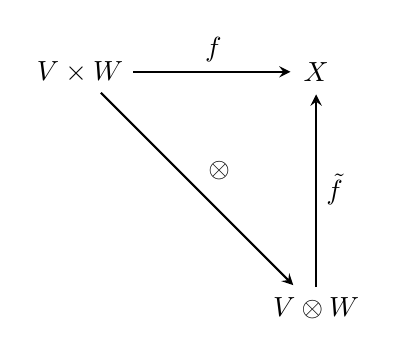
\begin{tikzpicture}[-,>=stealth,shorten >=1pt,auto,node distance=3cm, thick,main node/.style={scale=0.9,circle,draw,font=\sffamily\normalsize}]

		\node (1) []{$V \times W$};
		\node (2) [right of = 1]{$X$};
		\node (3) [below of = 2]{$V \otimes W$};

		\draw[->] (1) to node {$f$} (2);
		\draw[->] (1) to node {$\otimes$} (3);
		\draw[->] (3) to node[right] {$\tilde f$} (2);

		;
	\end{tikzpicture}
	\caption{The diagram of the definition above.}
\end{figure}


This definition is quite rigorous and dense, but a concrete example will make it clear. First, we recall that a function $f$ is \tbf{linear} if it holds that

\begin{itemize}
	\item $f(x + y) = f(x) + f(y)$
	\item $f (\alpha x) = \alpha f(x)$
\end{itemize}

Then, for a function to be \tbf{bilinear} (or \tit{multilinear}, in general) we require $f$ to be linear in both of its arguments:

\begin{itemize}
	\item $f(x + x', y) = f(x, y) + f(x', y)$
	\item $f(x, y + y') = f(x, y) + f(x, y')$
	\item $f(\alpha x, y) = \alpha f(x, y) = f(x, \alpha y)$
\end{itemize}

From this definition, we immediately point out that the tensor product $\otimes$ satisfies

\begin{itemize}
	\item $(v + v') \otimes w = v \otimes w + v' \otimes w$
	\item $v \otimes(w + w') = v \otimes w + v \otimes w'$
	\item $(\alpha v) \otimes w = v \otimes (\alpha w)$
\end{itemize}

We may call the first two as \tit{distributive properties}. Let's consider an example we already presented in the first chapter of the notes. At the start of our discussion we \curlyquotes{defined} the tensor product between two vectors $\rmat{a \\ b}$ and $\rmat{c \\ d}$ as follows $$\rmat{a \\ b} \otimes \rmat{c \\ d} := \rmat{ac \\ ad \\ bc \\ bd}$$ Now that we know what true definition is, we can apply it to understand why this is the case. First, we can assume that $\rmat{a \\ b}, \rmat{c \\ d} \in \R^2$ therefore $V = W = \R^2$. Therefore, our tensor product will have the signature $$\func{\otimes}{\R^2 \times \R^2}{\R^2 \otimes \R^2}$$ Now, we observe that the output space $V \otimes W$ is a vector space that has $$\mathcal B_{V \otimes W} := \{f_i  \otimes g_j \mid f_i \in \mathcal B_V, g_j \in \mathcal B_W\}$$ as a basis. In particular, this means that $$\mathcal B_{\R^2 \otimes \R^2} = \{e_1 \otimes e_1, e_1 \otimes e_2, e_2 \otimes e_1, e_2 \otimes e_2\}$$ is a basis for $\R^2 \otimes \R^2$. In fact, it is not diffcult to prove that $\R^4 \cong \R^2 \otimes \R^2$ by mapping the canonical basis of $\R^4$ to $\mathcal B_{\R^2 \otimes \R^2}$. Let $\varphi$ be the isorphism between the two. Then, by bilinearity of $\otimes$ we have that
\begin{equation*}
	\begin{split}
		\varphi \rbk{\rmat{a                                                                                                                               \\ b} \otimes \rmat{c \\ d}} & =   \varphi \rbk{(a e_1 + b e_2) \otimes (c e_1 + d e_2) }\\
		 & = \varphi \rbk{a c (e_1 \otimes e_1) + ad (e_1 \otimes e_2) + bc (e_2 \otimes e_1) + bd (e_2 \otimes e_2) }                                     \\
		 & = ac \cdot \varphi(e_1 \otimes e_1) + ad \cdot \varphi(e_1 \otimes e_2) + bc \cdot \varphi(e_2 \otimes e_1) + bd \cdot \varphi(e_2 \otimes e_2) \\
		 & = ac \cdot e_1 + ad \cdot e_2 + bc \cdot e_3 + bd \cdot e_4                                                                                     \\
		 & = \rmat{ac                                                                                                                                      \\ ad \\ bc \\ bd} \\
	\end{split}
\end{equation*}
Thus, in our example we have that $\tilde f = \varphi$ itself and $X = \R^4$, indeed $f = \varphi \circ \otimes$ is a function that maps pairs of two-dimensional vectors in $\R^2 \times \R^2$ into 4-dimensional vectors inside $\R^4$. This example also shows that the definition of tensor product does not depend on the choice of the vector space $X$, and for our purposes it is practical to choose a vector space that is isomporphic to $V \otimes W$.

What is the purpose of the tensor product in the first place? Given a vector space $V$, let $$\mbox{Functions}(V) := \{\func{f}{V}{K}\}$$ be the set of functions from $V$ to some other field $K$. It can be proven that this set forms a \tbf{vector space}. Then, the \tbf{tensor product} is the mathematical object that enables the following $$\mbox{Functions}(V \times W) = \mbox{Functions}(V) \otimes \mbox{Functions}(W)$$ This property is very useful as it allows to reason about functions on $V \times W$ not as a completely new object, but by studying it in terms of functions on $V$ and $W$ individually. In general, it allows to deal with objects that are \curlyquotes{more managable}. For instance, in our previous example the pair $\rbk{ \rmat{a \\ b}, \rmat{c \\ d}} \in \R^2 \times \R^2$ lies on a \tit{grid}, while an object $\rmat{ac \\ ad \\ bc \\ bd} \in \R^4$ is just a 4-dimensional vector.

Lastly, from the definition we observe that $$\dim(V \otimes W) = \dim V \cdot \dim W$$ indeed $V$ and $W$ can have different dimensions. For instance, a pair of vectors $(v, w) \in \R^2 \times \R^3$ lies in a 5-dimensional space, since $$\dim(V \times W) = \dim V + \dim W$$ however the tensor product generates a bigger space of size $$\dim (\R^2 \otimes \R^3) = \dim \R^2 \cdot \dim \R^3 = 2 \cdot 3 = 6$$ Indeed, we have that $$\R^2 \times \R^3 \cong \R^5 \quad \quad \R^2 \otimes \R^3 \cong \R^6$$

Consider any two vectors $v \in V$ and $w \in W$, and suppose that $n := \dim V$ and $m := \dim W$. Then, we can describe them in terms of $\mathcal B_V$ and $\mathcal B_W$, respectively, as follows: $$v = \sum_{i = 1}^n{\alpha_i f_i} \quad \quad w = \sum_{j = 1}^m{\beta_j g_j}$$ Then, by the distributive properties in the definition we have that
\begin{equation*}
	\begin{split}
		v \otimes w & = \rbk{\sum_{i = 1}^n{\alpha_i f_i}} \otimes \rbk{\sum_{j = 1}^m{\beta_j g_j}} \\
		            & = \sum_{i = 1}^n{\sum_{j = 1}^m{\alpha_i \beta_j (f_i \otimes g_j)}}
	\end{split}
\end{equation*}
which indeed is a vector that lies inside $V \otimes W$ since $(f_i \otimes g_j) \in \mathcal B_{V \otimes W}$. Then, if the basis of choice of the output set $X$ is the canonical basis, we observe that
\begin{equation*}
	\begin{split}
		\varphi(v \otimes w) & = \varphi \rbk{ \sum_{i = 1}^n{\sum_{j = 1}^m{\alpha_i \beta_j (f_i \otimes g_j)}}} \\
		                     & =  \sum_{i = 1}^n{\sum_{j = 1}^m{\alpha_i \beta_j \varphi(f_i \otimes g_j)}}        \\
		                     & =  \sum_{i = 1}^n{\sum_{j = 1}^m{\alpha_i \beta_j e_{(i - 1)m + j}}}                \\
		                     & = \rmat{\alpha_1 \beta_1                                                            \\ \alpha_1 \beta_2 \\ \vdots \\ \alpha_1 \beta_m \\ \alpha_2 \beta_1 \\ \vdots \\ \alpha_n \beta_m} \in \R^{n \cdot m} \\
	\end{split}
\end{equation*}
where the last column vector contains \tit{all} the pairs $(\alpha_i, \beta_j)$ --- note that $\R^{n \cdot m} \neq \R^{n \times m}$, as the latter denotes the space of real-valued matrices of dimension $n \times m$. Again, we underline that we arbitrarily chose the space $\R^{n \cdot m}$, but we could have chosen \tit{any} space of dimension $n \cdot m$ as output --- even $\R^{n \times m}$! A concrete example will clarify: consider two spaces $V = \R^2$ and $W = \R^{2 \times 2}$. Then, any element $v \in \R^2$ has the form $v = \rmat{a \\ b}$ while any matrix of $A \in \R^{2 \times 2}$ looks like $A = \rmat{c & d \\ e & f}$. If we want to compute $v \otimes A$, we can project it onto any space that has dimension $$\dim(\R^2 \otimes \R^{2 \times 2}) = \dim \R^2 \cdot \dim \R^{2 \times 2} = 2 \cdot 4 = 8$$ Here are some examples of the possible outputs of $v \otimes A$ depending on the choice of the output space: $$\rmat{ac \\ ad \\ ae \\ af \\ bc \\ bd \\ be \\ bf} \in \R^8 \quad \quad \rmat{ac & ad & ae & af \\ bc & bd & be & bf} \in \R^{2 \times 4} \quad \quad \rmat{ac & bc \\  ad & bd \\  ae & be \\ af & bf} \in \R^{4 \times 2}$$

\subsection{Kronecker product}

To conclude this chapter, let's look at the tensor product from the point of view of quantum computing. Until now, we presented examples regarding real-valued vectors, however, when talking about Hibert spaces in quantum computing we often need \tit{complex} values, as we already know. Consider a qubit $$\ket \psi = \alpha \ket 0 + \beta \ket 1$$ From this very formulation, we see that we are representing $\ket \psi$ under the \tbf{computational basis} $\{\ket 0, \ket 1\}$ we already encountered. However, since $\alpha, \beta \in \C$ this implies that $\ket \psi \in \C^2$. Now, consider a unitary operator acting on one qubit, for example the Hadamard gate $$H = \dfrac{1}{\sqrt 2} \rmat{1 & 1 \\ 1 & -1}$$ Our next goal is to compute $H \otimes H$. Clearly $H \in \C^{2 \times 2}$, therefore $H \otimes H \in \C^{2 \times 2} \otimes \C^{2 \times 2}$ which yields a space isomporphic to $\C^{16}$. However, since $H$ is a matrix it is not convenient to express the result inside $\C^{16}$, so we usually represent it inside $\C^{4 \times 4}$, which is still isomporphic to $\C^{16}$. After some calculations, we can show that $$H \otimes H = \dfrac{1}{2} \rmat{1 & 1 & 1 & 1 \\ 1 & -1 & 1 & -1 \\ 1 & 1 & -1 & -1 \\ 1  & -1 & -1 & 1}$$ However, we notice an interesting pattern in this result: this $4 \times 4$ matrix is essentially split into 4 sections that are \curlyquotes{multiples} of $H$ $$H \otimes H = \dfrac{1}{\sqrt 2} \rmat{1 \cdot H & 1 \cdot H \\ 1 \cdot H & -1 \cdot H}$$ In fact, for any two matrices $$A = \rmat{a & b \\ c & d} \quad \quad B = \rmat{e & f \\ g & h}$$ it holds that $$A \otimes B = \rmat{a B & b B \\ c B & d B } = \rmat{ae & af & be & bf \\ ag & ah & bg & bh \\ ce & cf & de & df \\ cg & ch & dg & dh}$$

We are finally ready to provide the formulation of the tensor product we will adopt for our purposes.

\begin{frameddefn}{Kronecker product}
	Given two matrices $A \in \mathbb F^{m \times n}$ and $B \in \mathbb F^{p \times q}$ defined over some field $\mathbb F$, the \tbf{Kronecker product} between $A$ and $B$ defines $A \otimes B$ as follows $$A \otimes B = \rmat{a_{11} B & \ldots & a_{1n}B \\ \vdots & \ddots & \vdots \\ a_{m1} B & \ldots & a_{mn} B} \in \F^{mp \times nq}$$
\end{frameddefn}

As an example, we observe that $$\rmat{a \\ b} \otimes \rmat{c \\ d} = \rmat{a \rmat{c \\ d} \\ b \rmat{c \\ d}} = \rmat{ac \\ ad \\ bc \\ bd}$$ which matches our previous results. From now on, we will assume that the output of any tensor product is in this form. Most importantly, through the Kronecker product the following property holds, which will be used extensively through these notes.

\begin{framedprop}[label={broken tensor}]{}
	For any field $\mathbb F$, given two matrices $A$ and $B$ and two vectors $v$ and $w$ such that $$A \in \mathbb F ^{m \times n} \quad B \in \mathbb F^{p \times q} \quad v \in \mathbb F^n \quad w \in \mathbb F^q$$ it holds that $$(A \otimes B)(v \otimes w) = Av \otimes Bw$$
\end{framedprop}

\begin{framedprop}[label={tensor adj}]{}
	For any two matrices $A$ and $B$ defined over a Hilbert space, it holds that $$(A \otimes B)^\dag = A^\dag \otimes B^\dag$$
\end{framedprop}

Another very important property of the tensor product is the way it behaves together with our scalar product.

\begin{framedprop}[label={tensor scalar}]{}
	For any four vectors $\ket a, \ket c \in \mathcal H_1$ and $\ket b, \ket d \in \mathcal H_2$ of two Hilbert spaces $\mathcal H_1$ and $\mathcal H_2$, it holds that $$\braket{a \otimes b| c \otimes d} = \braket{a|c} \braket{b|d}$$
\end{framedprop}

As a final note, if $U$ is a matrix (or a vector), we will write $$U^{\otimes n} = \underbrace{U \otimes \ldots \otimes U}_{n \ \mathrm{times}}$$ similar to the usual product $$U^{n} = \underbrace{U \cdot \ldots \cdot U}_{n \ \mathrm{times}}$$

\section{Exercises}

\begin{framedprob}{}
	Given $n$ qubits $\{q_i\}_{i = 1}^n$, show that $$\norm{\bigotimes_{i = 1}^n q_i} = 1$$
\end{framedprob}

\solution{
First, we observe that by \cref{tensor scalar} it immediately follows that for any set of vectors ${\{x_i\}^n}_{i = 1}$ and ${\{y_i\}^n}_{i = 1}$ it holds that $$\braket{a|b} = \prod_{i = 1}^n \braket{x_i|y_i}$$ From this observation, we conclude that it holds that $$\abk{ \bigotimes_{i = 1}^n x_i\middle|\bigotimes_{i = 1}^n y_i} = \prod_{i = 1}^n{\braket{x_i|y_i}}$$ From this observation, we conclude that

\begin{equation}
	\begin{alignedat}{2}
		\norm{\bigotimes_{i = 1}^n q_i}^2 & = \abk{\bigotimes_{i = 1}^n q_i \middle| \bigotimes_{i = 1}^n q_i} &                                            \\
		                                  & = \prod_{i = 1}^n \braket{q_i |q_i}                                                                             \\
		                                  & = \prod_{i = 1}^n \norm{q_i}^2                                     &                                            \\
		                                  & = \prod_{i = 1}^n 1                                                & \quad \quad (\mbox{since they are qubits}) \\
		                                  & = 1
	\end{alignedat}
\end{equation}
which ultimately concludes that $$\norm{\bigotimes_{i = 1}^n q_i} = 1$$
}

\begin{framedprob}{}
	Let $\{f_i\}_{i = 1}^n$ be an orthonormal basis of a vector space $V$, and fix a vector $u \in V$; then, consider $$u_V := \sum_{i = 1}^n{\braket{f_i|u} f_i}$$ Prove that the definition of $u_V$ does not depend on the choice of $\{f_i\}_{i = 1}^n$
\end{framedprob}

\solution{
By way of contradiction, suppose that there is an orthonormal basis $\{g_i\}_{i = 1}^n$ of $V$ such that $$\sum_{i = 1}^n \braket{f_i|u} \ket {f_i} \neq \sum_{i = 1}^n \braket{g_i|u} \ket{g_i}$$ Then, we have that
\begin{equation*}
	\begin{split}
		     & \sum_{i = 1}^n \braket{f_i|u} \ket {f_i} \neq \sum_{i = 1}^n \braket{g_i|u} \ket{g_i}        \\
		\iff & \sum_{i = 1}^n \ket {f_i}\braket{f_i|u}  \neq \sum_{i = 1}^n \ket{g_i}\braket{g_i|u}         \\
		\iff & \sum_{i = 1}^n \rbk{\ket{f_i} \braket{f_i|u} - \ket{g_i} \braket{g_i|u}} \neq 0              \\
		\iff & \sum_{i = 1}^n  \rbk {\ket{f_i} \bra{f_i} - \ket{g_i} \bra{g_i}} \ket u \neq 0               \\
		\iff & \rbk{\sum_{ i = 1}^n \ket{f_i} \bra{f_i} - \sum_{i = 1}^n \ket{g_i} \bra{g_i}} \ket u \neq 0 \\
		\iff & (P_V - P_V) \ket u  \neq 0                                                                   \\
		\iff & 0 \neq 0
	\end{split}
\end{equation*}
which is clearly a contradiction $\lightning$.
}

\begin{framedprob}[label={converse proj}]{}
	Show that if a matrix $P$ is both idempotent and Hermitian, it must be a projector.
\end{framedprob}

\solution{
    By Hermiticity, we know that $P$ admit a \nameref{spectral decomp}, i.e. $$P = \sum_{i = 1}^n{\lambda_i \ket{\lambda_i} \bra{\lambda_i}}$$ Now consider the following claim.

    \claim{
        If $P$ is an idempotent operator, its only possible eigenvalues are 0 and 1.
    }{
        By definition $v$ is an eigenvalue of $P$ associated to the eigenvector $\lambda$ if it holds that $$Pv = \lambda v$$ Hence, we observe that $$P^2 v = P (P v) = P (\lambda v) = \lambda Pv = \lambda(\lambda v) = \lambda^2 v$$ and therefore we have that $$\lambda^2 v = P^2 = Pv = \lambda v$$ which implies that $$\lambda^2v - \lambda v = 0 \iff (\lambda^2 - \lambda)v = 0$$ Finally, since $v$ is an eigenvector it holds that $v \neq 0$, therefore it must be that the last equation is true only if $$\lambda^2 - \lambda = 0 \iff \lambda = 0 \lor \lambda = 1$$
    }

    From this claim, we immediately obtain that each $\lambda_i$ is either 0 or 1, which means that its spectral decomposition can be written as $$P = \sum_j \ket{\lambda_j} \bra{\lambda_j}$$ for some non-zero eigenvalues $\lambda_j$ of $P$. This formulation concludes that $P$ is indeed a projector.
}

\begin{framedprob}{}
    Given a unitary matrix $U$, show that $U^{\otimes n}$ is still unitary.
\end{framedprob}

\solution{
    The property follows immediately from \cref{broken tensor} and \cref{tensor adj}, since
    \begin{equation*}
        \begin{split}
            U^{\otimes n} (U^{\otimes n})^\dag & = \rbk{ \bigotimes_{i = 1}^n U } \rbk{\bigotimes_{i = 1}^n U}^\dag \\ 
                                               & = \rbk{\bigotimes_{i = 1}^n U} \rbk{\bigotimes_{i = 1}^n U^\dag} \\ 
                                            & = \bigotimes_{i = 1}^n U U^\dag \\ 
                                            & = \bigotimes_{i = 1}^n I \\ 
                                             & = I
        \end{split}
    \end{equation*}
    The product $(U^{\otimes n})^\dag U^{\otimes n}$ can be proved analogously.
}

\begin{framedprob}{}
    Prove the triangular inequality.
\end{framedprob}

\solution{
    Consider two vectors $u$ and $v$ in some scalar product vector space; we must show that $$\norm{u + v} \le \norm u + \norm v$$ First, we observe that
    \begin{equation*}
        \begin{split}
            \norm{u + v}^2 & = \braket{u + v|u + v} \\ 
                           & = \braket{u + v|u} + \braket{u + v|v} \\ 
                           & = \braket{u|u} + \braket{v|u} + \braket{u|v} + \braket{v|v} \\ 
                           & = \norm u^2 + \braket{u|v} + \overline{\braket{u|v}} + \norm v^2
        \end{split}
    \end{equation*}
    Now, consider the following claim.

    \claim{
        For any complex number $z \in \C$ it holds that $z + \overline z = 2 \Re(z)$.
    }{
        The statement can be easily proven as follows: $$z + \overline z = \Re(z) + \Im(z) + \Re(z) - \Im(z) = 2 \Re(z)$$
    }

    From this claim, we can proceed as follows:
    \begin{equation*}
        \begin{alignedat}{2}
            \norm{u + v}^2 & = \norm u^2 + \braket{u|v} + \overline{\braket{u|v}} + \norm v^2 & \\ 
                           & = \norm u^2 + 2 \Re(\braket{u|v}) + \norm v^2 & \\ 
                           & \le \norm u^2 + 2 \abs{\braket{u|v}} + \norm v^2 & \\ 
                           & \le \norm u^2 + 2 \sqrt{\braket{u|u} \cdot \braket{v|v}} + \norm v^2 & \quad \quad (\mbox{by the \nameref{cs ineq}}) \\ 
                           & = \norm u^2 + 2 \sqrt{\braket{u|u}} \cdot \sqrt{\braket{v|v}} + \norm v^2 &  \\ 
                           & = \norm u^2 + 2 \norm u \norm v + \norm v^2 & \\ 
                            & = (\norm u + \norm v ) ^2 & \\ 
        \end{alignedat}
    \end{equation*}
    Then, since the vector norm is defined positive we ultimately conclude that $$\norm{u + v}^2 \le (\norm u + \norm v)^2 \implies \norm{u + v} \le \norm u + \norm v$$
}

\begin{framedprob}{}
    Prove the second property of the \nameref{spectral thm}, i.e. that the eigenvalues of a unitary operator are complex values of modulus 1.
\end{framedprob}

\solution{
    Let $U$ be a unitary transformation defined over some Hilbert space $\mathcal H$; by \cref{unitary alt def} we know that $$\forall x, y \in \mathcal H \quad \braket{Ux|Uy} = \braket{x|y}$$ Let $v \in \mathcal H$ be an eigenvector of $U$, i.e. there exists $\lambda \in \mbox{sp}(U)$ such that $$U \ket v = \lambda v$$ Then, we have that
    \begin{equation*}
        \begin{split}
            \braket{v|v} & = \braket{Uv|Uv} \\ 
                         & = \braket{\lambda v|\lambda v} \\
                            & = \overline \lambda \bra v \cdot \lambda \ket v \\ 
                            & = \abs{\lambda}^2 \braket{v|v}
        \end{split}
    \end{equation*}
    and since $v \neq 0$ because it is an eigenvector of $U$ we have that $$\braket{v|v} = \abs{\lambda}^2 \braket{v|v} \iff 1 = \abs{\lambda}^2 \implies \abs{\lambda} = 1$$
}

\begin{framedprob}{}
    Show that if an operator is unitary, it must be linear.
\end{framedprob}

\solution{
    Let $U$ be a unitary transformation defined over some Hilbert space $\mathcal H$; by \cref{unitary alt def} we know that $$\forall x, y \in \mathcal H \quad \braket{Ux|Uy} = \braket{x|y}$$ Fix three vectors $x, y, z \in \mathcal H$ and two complex values $\alpha, \beta \in \C$; then, by definition of scalar product we have that
    \begin{equation*}
        \begin{split}
            \braket{U(\alpha x + \beta y)|z} & = \braket{\alpha x + \beta y|U^\dag z} \\  
                                             & = \overline \alpha \braket{x|U^\dag z} + \overline \beta \braket{y| U^\dag z} \\ 
                                             & = \braket{\alpha Ux|z}  + \braket{\beta Uy|z} \\ 
                                              & = \braket{\alpha U x + \beta U y|z} \\
        \end{split}
    \end{equation*}
    Now, consider the following property of the scalar product.

	\claim{
		Given $x, y \in \mathcal H$, if  $\braket{x|z} = \braket{y|z}$ for all $z \in \mathcal H$, then $x = y$.
	}{
		Fix a vector $z \in \mathcal H$; we observe that
		\begin{equation*}
			\begin{split}
				     & \braket{x|z} = \braket{y|z}     \\
				\iff & \braket{x|z} - \braket{y|z} = 0 \\
				\iff & \braket{x - y|z} = 0
			\end{split}
		\end{equation*}
		However, if this is true for every vector $z \in \mathcal H$ it means that the vector $x - y$ is orthogonal to every vector in $\mathcal H$, which must imply that $x - y$ is the 0 vector, thus $$x - y = 0 \iff x = y$$
	}
        
        Then, from the previous observation we have $$\forall x, y, z \in \mathcal H , \alpha, \beta \in \C \quad \braket{U(\alpha x + \beta y)|z} = \braket{\alpha Ux + \beta Uy|z}$$ and this last claim concludes that $$U(\alpha x + \beta y) = \alpha U x + \beta U y$$ meaning that $U$ is indeed linear.
}
